\documentclass[12pt]{article}

\usepackage[a4paper,margin=1in]{geometry}
\usepackage{amsmath,amssymb,amsthm}
\usepackage{graphicx}
\usepackage{booktabs}
\usepackage{float}
\usepackage{enumitem}
\usepackage{hyperref}
\usepackage{xcolor}
\usepackage{array}
\usepackage{tocloft}
\setlength{\emergencystretch}{4em}

\setcounter{tocdepth}{1}
\renewcommand{\contentsname}{Kézirat-útiterv}
\renewcommand{\abstractname}{Kivonat}
\renewcommand{\refname}{Hivatkozások}
\renewcommand{\cfttoctitlefont}{\Large\bfseries}
\renewcommand{\cftsecfont}{\normalfont}
\renewcommand{\cftsecpagefont}{\normalfont}
\renewcommand{\cftsecleader}{\cftdotfill{\cftdotsep}}
\setlength{\cftbeforesecskip}{2pt}
\setlength{\cftsecnumwidth}{2.8em}

\hypersetup{
  colorlinks=true,
  linkcolor=black,
  citecolor=blue!50!black,
  urlcolor=blue!50!black
}

\newtheorem{definition}{Definíció}
\newtheorem{postulate}{Posztulátum}
\newtheorem{proposition}{Állítás}
\newtheorem{lemma}{Lemma}
\newtheorem{conjecture}{Sejtés}

\newcommand{\T}{\mathcal T}
\newcommand{\Ssrc}{\mathcal S}
\newcommand{\RTspace}{\mathfrak R_{\tau}}
\newcommand{\Rmap}{\rho_{\tau}}
\newcommand{\Ui}{U_i}
\newcommand{\Mta}{M_{\tau}}
\newcommand{\Obs}{\mathcal O}
\newcommand{\Def}{\mathcal D}
\newcommand{\Rel}{\mathcal J}
\newcommand{\Null}{\mathcal N}
\newcommand{\Ker}{\operatorname{Ker}}
\newcommand{\im}{\operatorname{im}}
\newcolumntype{L}[1]{>{\raggedright\arraybackslash}p{#1}}

\title{\textbf{Tau Core: időtlen morfológiai kiolvasási keret az emergens fizikai leírásokhoz}\\
\large Foundation Paper I -- magyar változat}
\author{Olcsák József\\
\small Független kutató}
\date{Draft v0.2 -- 2026}

\begin{document}

\maketitle

\begin{abstract}
\noindent\textbf{Cél.}
A Tau Core ebben a kéziratban óvatos alapozó keretként jelenik meg, nem
befejezett fizikai elméletként.  A kiinduló lehetőség az, hogy a szokásos
dinamikus fizika nem feltétlenül primitív téridőn zajló időfejlődés, hanem
egy mélyebb, időtlen válaszszerkezet effektív kiolvasása.

\medskip
\noindent\textbf{Formai gerinc.}
\[
  s \longmapsto \Rmap(s) \longmapsto U_i^{\Mta}(\Rmap(s)),
\]
ahol \(s\) parent-oldali forrásmag, \(\Rmap(s)\) endpoint-vak Tau-válasz, és
\(\Mta\) a Tau-oldali morfológiai test, míg \(U_i^{\Mta}\)
morfológia-kondicionált szektor-kiolvasás: például téridő-, megfigyelői idő-,
kvantum-, gravitációs vagy tömeg/forrás-kiolvasás.

\medskip
\noindent\textbf{Hatókör.}
A központi állítás architekturális.  A formalizmus nyelvet ad a definíciók,
posztulátumok, feltételes következmények, toy mechanizmusok és későbbi
empirikus tesztek szétválasztására.  A kézirat elhatárolja a keretet a
blokk-univerzum ontológiától és a szokásos téridő-mezőelmélettől, definiálja a
Tau-oldali morfológiai testet, hét alapozó posztulátumot fogalmaz meg, a
relift-kudarc nyelvén bevezeti a kiolvasás-relatív rejtett defektust, és véges
toy modelleket ad a rejtettségre és az effektív readout-időre.
Ezt a kéziratot alapnyelvi és állításihatár-paperként kell értékelni, nem
fenomenológiai vagy empirikus eredménypaperként.

\medskip
\noindent\textbf{Határ.}
A fő blokkolók is explicit módon szerepelnek.  A paper nem vezeti le az
általános relativitás\-elméletet, a kvantummechanikát, a Born-szabályt, a
kvantum\-térelméletet, a Standard Modellt, a sötét anyagot, a sötét energiát
vagy egy fizikai parent akciót.  Ez pozíció-paper és formai sejtésváz, nem
empirikus bizonyíték új fizikai törvényre.
\end{abstract}

\clearpage
\tableofcontents
\clearpage

\section{Cél és állítási határ}

Ez a kézirat az első római számozású Tau Core alapozó paper.  Elkülönül az
arab számozású Tau Core papersorozattól, amely szűkebb empirikus vagy
protokoll-csomagokra szolgál.  Itt a cél alapvetőbb: a jelenlegi alapnyelvet
olyan formában rögzíteni, amely kritizálható, összehasonlítható és finomítható.

Beküldési megjegyzés: ezt a kéziratot alapnyelvi és állításihatár-paperként
kell értékelni, nem fenomenológiai vagy empirikus eredménypaperként.

Az állítási határ szándékosan szűk.  A paper formai architektúrát és
auditfegyelmet javasol, nem validált fizikai modellt.  Olyan szókészletet ad,
amelyben a téridő, kvantumelmélet, gravitáció és sötétszektor-nyelv későbbi
kérdései feltehetők anélkül, hogy a téridőbeli időfejlődést primitív szintnek
vennénk.  A fő kizárások az alábbi dobozban röviden, a kézirat végén pedig
tételesen szerepelnek.

\begin{center}
\fbox{\begin{minipage}{0.90\linewidth}
\textbf{Reviewer-facing claim box.}
Ez a paper formai readout-architektúrát és bukási fegyelmet állít.
Nem állít empirikus validációt, új erőt, sötétanyag-helyettesítést,
GR/QM/Standard-Model levezetést.
Bármely későbbi ág előléptetéséhez source-freeze, quotient safety,
ismert-limit visszanyerés, endpoint-vak predikció vagy kizárás, valamint
releváns holdout/kontroll túlélés kell.
\end{minipage}}
\end{center}

A központi gondolat egy sorban:
\begin{equation}
  s \longmapsto \Rmap(s) \longmapsto U_i^{\Mta}(\Rmap(s)).
  \label{eq:core-spine-hu}
\end{equation}
Az első nyíl nem időfejlődés.  Parent-oldali válaszreláció.  A második nyíl
kiolvasás.  Fizikai elmélet csak akkor jelenik meg, ha egy kiolvasás
megadta a kodomént, a null-politikát, a closure-tesztet és a validációs határt.
Ha \(\Mta\) a deklarált forrásosztály által rögzített, a felső indexet gyakran
elhagyjuk, és \(U_i\)-t írunk \(U_i^{\Mta}\) helyett.

Determinisztikus ágban írható:
\[
  \Rmap:\Ssrc\to\RTspace.
\]
Relációs ágban ugyanez a jelölés relációt jelent:
\[
  \Rmap\subseteq\Ssrc\times\RTspace,
\]
vagy ekvivalensen halmazértékű válaszszabályt:
\[
  \Rmap:\Ssrc\to\mathcal P(\RTspace).
\]
Ilyenkor az ágnak deklarálnia kell, hogy a teljes admisszibilis válaszosztályt
használja-e, vagy endpoint-vak source-freeze szabály választ reprezentánst.

Ekvivalensen a paper a következő alapozó csomaggal dolgozik:
\[
  \mathfrak T
  =
  (\Ssrc,\RTspace,\Rmap,\Mta,\{U_i\},\{N_i\},\{J_i\}).
\]
Itt \(\Ssrc\) forrásdomén, \(\RTspace\) formai válaszdomén, \(\Rmap\)
térkép, reláció vagy halmazértékű válaszszabály, \(\Mta\) morfológiai test,
\(U_i\) szektor-readout, \(N_i\) null/quotient politika, \(J_i\) opcionális
relift.  Ez a csomag későbbi ágak szervező objektuma, nem annak bizonyítása,
hogy a természet ilyen csomagot használ.

Informális Tau Core beszélgetésekben a \emph{Tau Core alapmező} kifejezés erre
a parent-oldali válaszszubsztrátumra utal: ebben a paperben
\((\Ssrc,\RTspace,\Rmap)\), a morfológiai testtel \(\Mta\) együtt.  A
kifejezés heurisztikus.  Itt nem fizikai mezőt jelent akcióval,
mozgásegyenlettel, egységekkel, stressz-energiával vagy empirikus kalibrációval.

\paragraph{Módszertani megjegyzés.}
A kézirat AI-segített elméleti kutatási munkafolyamatban készült.  Az
AI-munkafolyamat nem bizonyíték semmilyen fizikai állításra; csak a drafting
és audit folyamat része.

\begin{figure}[t]
  \centering
  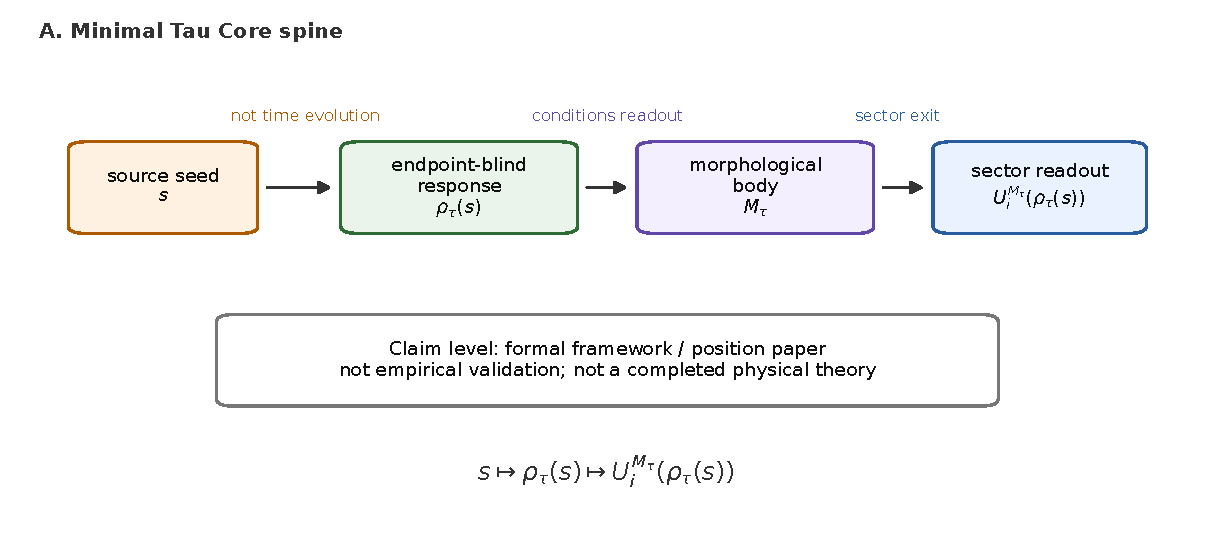
\includegraphics[width=0.95\linewidth]{figures/fig_core_spine.pdf}
  \caption{A Foundation Paper I-ben használt minimális Tau Core gerinc.  A
  parent-oldali forrásmag \(s\) endpoint-vak Tau-választ \(\Rmap(s)\) indukál.
  A Tau-oldali morfológiai test \(\Mta\) kondicionálja a szektor-kiolvasásokat
  \(U_i\).  Ez formai architektúra, nem empirikus validáció.}
  \label{fig:core-spine-hu}
\end{figure}

Ezért a paper inkább formai sejtés- vagy pozíció-paper, mint fenomenológiai
paper.  Akkor hasznos, ha a későbbi kutatási programot jobban cáfolhatóvá
teszi.  Egy tág ontológia, amely nem fordítható fagyasztott forrásszabályokra,
null-tesztekre vagy endpoint-vak előrejelzésekre, fizikaként nem hasznos.

\section{Olvasói útiterv}

A papernek két feladata van.  Először: rögzíti a későbbi Tau Core munka
szókészletét.  Másodszor: kimondja, hogy ez a szókészlet mit nem bizonyít.

\begin{center}
\small
\begin{tabular}{L{0.23\linewidth}L{0.43\linewidth}L{0.22\linewidth}}
\toprule
Rész & Szerep & Állítási szint\\
\midrule
Nyitó részek & Motiváció, név, viszony a blokk-univerzumhoz és a téridő-mezőképhez & Pozicionálás\\
Alapszókészlet & Parent-válasz, morfológiai test, kiolvasás, relift, defektus & Definíciók\\
Formai gerinc & Minimális kalkulus, forrásfegyelem, effektív readout-idő, posztulátumok & Keretposztulátumok\\
Toy réteg & Véges hidden-defect modell és morfológia/megfigyelői idő tisztázása & Toy mechanizmus\\
Határréteg & Kvantum, gravitáció, kozmológia, korábbi paperek és ellenvetések & Határkijelölés\\
Audit réteg & Érettségi checklist, alapozó sorozat, összegzés és nem-eredmények & Auditfegyelem\\
\bottomrule
\end{tabular}
\end{center}

A paper tehát gyenge állítási szinttől erősebb felé olvasandó.  A definíció nem
válik automatikusan feltevéssé; a feltevés nem válik levezetett törvénnyé; a
toy modell nem válik empirikus validációvá.  Későbbi paperek megpróbálhatnak
konkrét ágakat előléptetni, de Foundation Paper I ezeket az előléptetéseket
az állítási határán kívül tartja.

\section{Miért kell alapozó paper?}

A modern alapkutatás több iránya is megkérdőjelezi, hogy az idő, a téridő vagy
a lokális dinamika primitív legyen.  A kanonikus kvantumgravitációban ismert a
``problem of time'', ahol időtlen kényszeregyenlet mellett is megjelenhet
effektív dinamika \cite{WheelerDeWitt1967,Rovelli2004}.  A relációs idő
konstrukciói azt mutatják, hogy dinamika korrelációkon keresztül is leírható
\cite{PageWootters1983}.  Időtlen vagy konfigurációs-tér alapú nézetek is
léteznek \cite{Barbour1999}.  A thermal-time hipotézis különösen közeli
összehasonlítási pont, mert az időt állapotfüggőnek kezeli, nem külső
primitívumnak \cite{ConnesRovelli1994}.  A causal-set és generalizált
kvantummechanikai programok szintén olyan példák, ahol a primitív leírási
réteg változik meg, nem pusztán új tag kerül egy egyenletbe
\cite{Bombelli1987,Hartle1991}.  A kvantumrekonstrukciós programok pedig azt
mutatják, hogy a kvantumformalizmus nagy része operacionális elvekből
szervezhető \cite{Hardy2001,Chiribella2011,MasanesMueller2011}.  A constructor
theory módszertani összehasonlításként hasznos, mert fizikai tartalmat
lehetséges/lehetetlen transzformációkon keresztül próbál rögzíteni, nem egy
konkrét dinamikai egyenleten keresztül \cite{Deutsch2013,DeutschMarletto2015}.

A Tau Core nem állítja, hogy ezeket a programokat megoldja.  Más szervező
kérdést használ:
\begin{quote}
Kezelhetők-e a megfigyelt szektorleírások egy mélyebb parent-válasz
kiolvasásaiként, úgy, hogy az időfejlődés, a kvantumállapot, a gravitáció, a
tömeg és a megfigyelői idő effektív szektorleírások legyenek, ne primitív
kategóriák?
\end{quote}
Ez szándékosan tágabb kérdés, mint bármelyik egyedi ág.  Ha túl tág marad,
metafizikává válik.  A jelen paper célja ennek megakadályozása: megadja azokat
a minimális objektumokat, amelyek nélkül egy Tau Core állítás nem matematikailag
értelmes.

\section{A Tau Core név}

A ``Tau Core'' név történeti.  A program időalapú intuícióból indult: talán a
négydimenziós megfigyelő által látott idő nem primitív háttér, hanem vetített
válasz.  Ez magyarázza a \(\tau\) jelölést, amely fizikában gyakran időhöz vagy
sajátidőhöz kötődik.

A jelenlegi architektúrában azonban \(\tau\) nem közönséges időt jelent.  A
teória parent-state oldalát nevezi meg.  Az idő ebből az oldalból csak az egyik
lehetséges kiolvasás.
\begin{center}
\begin{tabular}{lll}
\toprule
Jel vagy kifejezés & Jelentés itt & Nem ezt állítjuk\\
\midrule
\(\tau\) & parent-state oldal & maga a közönséges idő\\
\(X_{\tau}\) & parent Tau-állapot & detektált fizikai mező\\
\(\Rmap(s)\) & endpoint-vak válasz & időfejlődés\\
\(U_{\rm time}\) & idő-kiolvasás & levezetett óraelmélet\\
\(\Mta\) & morfológiai test & megfigyelt 4D alak\\
\bottomrule
\end{tabular}
\end{center}

Így a teória idő-motivált, de nem idő-redukcionista.  Nem azt mondja, hogy
minden időből van.  Azt mondja, hogy az idő a kiolvasási oldalhoz tartozik,
míg \(\tau\) azt a mélyebb oldalt nevezi meg, ahonnan idő és más fizikai
szektorok kiolvashatók.

\section{Eltérés a blokk-univerzumtól}

A blokk-univerzum olvasat a négydimenziós téridőtörténetet végső objektumnak
tekinti.  Ez nem szalmabáb: a relativisztikus háttér Minkowski
négydimenziós téridő-formulációjával kezdődik \cite{Minkowski1909}, majd a
Rietdijk--Putnam--Maxwell érvelés a szimultaneitás relativitásából
négydimenzionalizmus vagy eternalizmus felé mutat
\cite{Rietdijk1966,Putnam1967,Maxwell1985,Thyssen2023RPM}.  A standard
filozófiai áttekintések a lét, keletkezés, eternalizmus és blokk-univerzum
vitáját tárgyalják \cite{Savitt2021,MarkosianSullivan2025,PetersonSilberstein2010,Thyssen2020}.

Egy tömör blokk-univerzum állítás:
\begin{equation}
  \text{Valóság}=M_{4D}.
\end{equation}
A Tau Core ezzel szemben egy jó négydimenziós blokkot kiolvasásként kezel:
\begin{equation}
  M_{4D}=U_{4D}^{\Mta}(\Rmap(s)).
  \label{eq:block-readout-hu}
\end{equation}
A különbségnek csak akkor van fizikai tartalma, ha a téridőblokkon túl további
nem-téridő readout-kényszerek source-frozen módon rögzíthetők.  Ha nincs
nem-téridő readout, amely ilyen korlátozást ad, akkor a különbség inkább
metafizikai átfogalmazás marad, nem fizikai ág.
A különbség nem kozmetikai.  A blokk-univerzumban a 4D objektum a végső színtér.
A Tau Core-ban ez a színtér egy readout eredménye.  A parent-válaszban lehetnek
olyan különbségek, amelyeket az egyik kiolvasás azonosít, a másik elfelejt, a
harmadik pedig effektív readout-változássá fordít.

\begin{figure}[t]
  \centering
  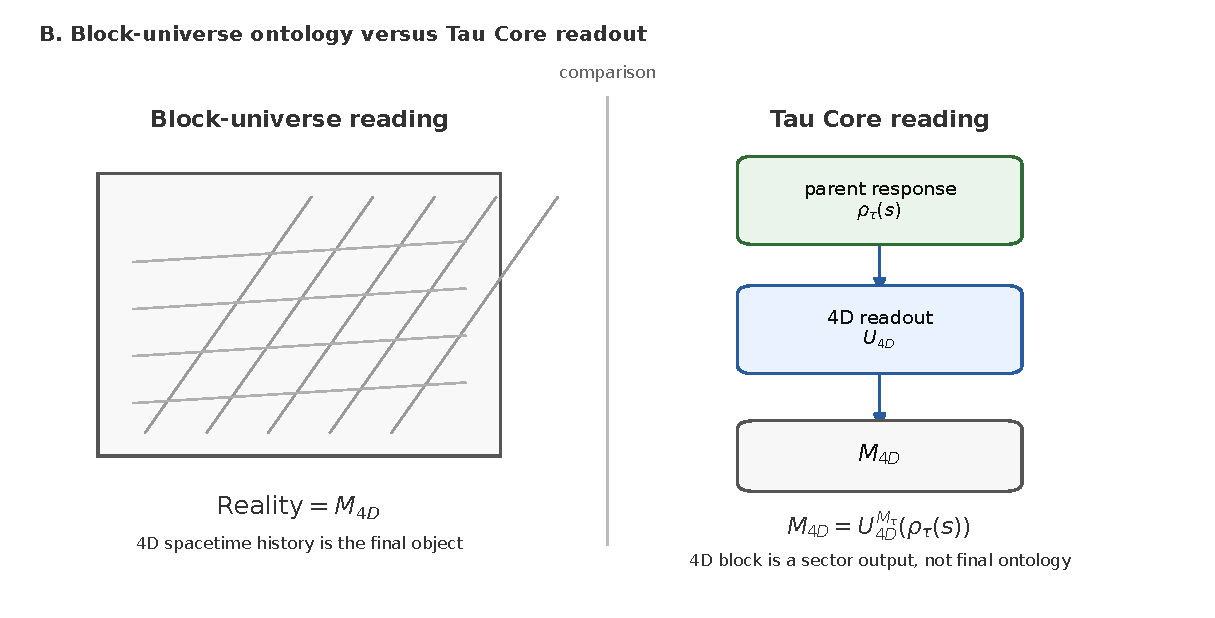
\includegraphics[width=0.95\linewidth]{figures/fig_block_vs_tau.pdf}
  \caption{A blokk-univerzum összehasonlítás.  Bal oldalt a standard 4D blokk
  olvasat, ahol a téridőtörténet a végső objektum.  Jobb oldalt a Tau Core
  pozíció: ugyanaz az effektív 4D blokk lehet egy mélyebb parent-válasz stabil
  kiolvasása.  Az ábra fogalmi különbséget mutat, nem az eternalizmus cáfolata.}
  \label{fig:block-vs-tau-hu}
\end{figure}

\section{Eltérés a szokásos téridő-mezőelmélettől}

Egy szokásos mezőelmélet téridőn adott mezővel indul:
\begin{equation}
  \phi:M_{4D}\to V,
\end{equation}
majd \(\phi(x,t)\) dinamikáját vizsgálja.  A Tau Core megfordítja a sorrendet:
\begin{equation}
  \phi_{\rm obs}(x,t)=U_{\phi}(\Rmap(s)).
  \label{eq:field-readout-hu}
\end{equation}
A megfigyelt mező kiolvasás.  A téridő-koordináták is a kiolvasási struktúra
részei.  Ez nem teszi rosszá a szokásos mezőelméletet.  Effektív, nagyon
sikeres leírássá teszi, miután egy adott szektor-kiolvasás stabil lett.

Ezért a Tau Core nem lehet sikeres pusztán attól, hogy új kiolvasási térképet
ír.  Fizikává csak akkor válik, ha visszaad ismert limiteket és túlél
empirikus kontrollokat.

\section{Alapszókészlet}

\begin{definition}[Parent forrásmag]
A parent forrásmag \(s\in\Ssrc\) Tau-oldali forrásadat.  Nem megfigyelt
endpoint, és nem választható ki abból a residualból, amelyet egy későbbi
kiolvasás magyarázni akar.
\end{definition}

\begin{definition}[Endpoint-vak Tau-válasz]
Endpoint-vak Tau-válasz egy
\[
  \Rmap:\Ssrc\to\RTspace
\]
térkép vagy reláció, amelynek inputja a parent forrásmag és az admisszibilis
parent-oldali kényszerek, nem pedig a megfigyelési endpoint.
Ha \(\Rmap\) reláció és nem egyértékű térkép, akkor \(\Rmap(s)\) az
admisszibilis válaszosztályt, vagy egy explicit source-freeze szabállyal
kiválasztott reprezentánst jelöl.  Endpoint residual nem használható a
reprezentáns kiválasztására.
\end{definition}

\begin{definition}[Morfológiai test]
A Tau-oldali morfológiai test \(\Mta\) az intrinsic strukturált test, amely a
kiolvasásokat kondicionálja.  Nem megfigyelt 4D morfológiai címke.  Tartalmazhat
szektor-, ág-, fal-, null-, Hessian-support-, admisszibilitási-, history- és
megfigyelő/útvonal-releváns szerkezetet.  A vetített morfológia csak egy
readout-handle erre a mélyebb testre.
\end{definition}

Foundation Paper I szintjén a minimális matematikai típus:
\[
  \Mta\in\mathcal M_\tau^{\rm adm},
\]
ahol \(\mathcal M_\tau^{\rm adm}\) admisszibilis morfológiai rekordok
deklarált osztálya.  Egy konkrét ág sematikusan például így instanciálhatja:
\[
  \Mta=(S,B,W,N,H,A;\Theta),
\]
ahol \(S\) szektorfelbontást, \(B\) ág/support szerkezetet, \(W\) fal- vagy
átmeneti szomszédságot, \(N\) null/protected struktúrát, \(H\)
Hessian-válasz supportot, \(A\) admisszibilitási kényszereket, \(\Theta\) pedig
opcionális interface/history/path adatot jelöl.  Ezért \(U_i^{\Mta}\) nem
dekoratív felső index: azt jelenti, hogy a readout egy típusozott családból
választódik:
\[
  U_i:\mathcal M_\tau^{\rm adm}\times\RTspace\to\Obs_i.
\]
Ez még mindig minimális típusdeklaráció, nem konstrukciós tétel
\(\mathcal M_\tau^{\rm adm}\)-re.

\begin{definition}[Kiolvasás]
Kiolvasás morfológia-kondicionált szektortérkép.  Ekvivalensen írható:
\[
  U_i^{\Mta}:\RTspace\to\Obs_i,
  \qquad\text{vagy}\qquad
  U_i:\mathcal M_\tau\times\RTspace\to\Obs_i.
\]
A kodomén lehet téridőleírás, időrend, kvantum-hozzáférési állapot,
gravitációs válasz, tömeg/forrás rekord vagy speciálisabb megfigyelhető
szerkezet.  Ha \(\Mta\) a deklarált forrásosztály által rögzített, röviden
\(U_i(r)\)-t írunk.  Minden kiolvasásnak saját null-iránya és validációs
határa van.
\end{definition}

\begin{table}[H]
\centering
\scriptsize
\begin{tabular}{L{0.16\linewidth}L{0.26\linewidth}L{0.23\linewidth}L{0.17\linewidth}}
\toprule
Readout-család & Parent/forrásosztály & Readout-alak & Minimális freeze-cél\\
\midrule
Téridő & lokális chart- és metrikus handle-ök & \(U_{4D}^{\Mta}(r)\) &
lokális intervallum vagy chart-limit\\
Megfigyelői idő & óra-, interface- és path-rekordok &
\(U_{\rm time}^{\Mta}(r,\mathcal O,\gamma)\) &
sajátidő-limit vagy fagyasztott path-korrekció\\
Kvantum-hozzáférés & hozzáférési, fázis-, kontextus- vagy kimenet-rekordok &
\(U_q^{\Mta}(r)\) &
normalizált hozzáférési valószínűségek vagy null/kontroll szabály\\
Gravitáció & gyenge-mezős, closure-, lencsézési vagy gyorsulási rekordok &
\(U_g^{\Mta}(r)\) &
Newtoni/GR-limit vagy quotientben látható residual\\
Tömeg/forrás & sűrűség-, forrásmérték-, flavor- vagy részecsketartalom-rekordok &
\(U_m^{\Mta}(r)\) &
konzervált forrásmérték vagy deklarált tömeg/forrás térkép\\
Kozmológia & web-, void-, path-, clock- vagy expanziós rekordok &
\(U_{\rm cosmo}^{\Mta}(r)\) &
FLRW/\(\Lambda\)CDM-limit vagy fagyasztott residual-csatorna\\
\bottomrule
\end{tabular}
\caption{Readout-családok és illusztratív parent/forrásosztályok.  A táblázat
nem vezeti le fizikailag a családokat; azt rögzíti, milyen minimális
könyvelés kell ahhoz, hogy egy ág több legyen puszta szókincsnél.  A freeze
célok szándékosan heterogén helyfoglalók.  Minden későbbi ágnak ezeket
operacionálisan definiált mennyiségekkel, egységekkel, bizonytalanságokkal,
nullmodellekkel és bukási szabályokkal kell kiváltania; itt még nem kalibrált
megfigyelhető mennyiségek.}
\label{tab:readout-families-hu}
\end{table}

\begin{definition}[Kereszt-skálájú readout-kompozíció]
A readout-családok ágszinten különbözők, de nem feltételezzük róluk, hogy
függetlenek.  Egy \(K_i\) jelölt kernel csak akkor admissible, ha a szomszédos
readout-családokhoz kötő source-, carrier-, quotient- és megfigyelhető
függéseket ellenőriztük, vagy a deklarált feltételek mellett expliciten
elhanyagolhatónak fagyasztottuk.  Másképp mondva: a Tau Core a fizikai
readoutokat kompatibilitással összekapcsolt kompozíciós hipergráfként kezeli,
nem izolált illesztési modulokként.
\end{definition}

Ez admissibility elv, nem unifikációs bizonyítás.  Nem vezet le kvantumgravitációt,
részecskefizikát, általános relativitást vagy kozmológiát.  A szerepe az, hogy
megtiltsa például egy galaxis-skálájú gravitációs kernel teljesen független
kezelését akkor, ha a megfigyelt carrier durvaszemcsés részecske-, tömeg-,
anyag-, sugárzási és path-readoutokból áll össze.  Double-counting ellen is
véd: két source-átfedő readout tag nem adható hozzá egymáshoz független
korrekcióként, hacsak a non-overlap és quotient-láthatóság nincs deklarálva.

\begin{figure}[t]
  \centering
  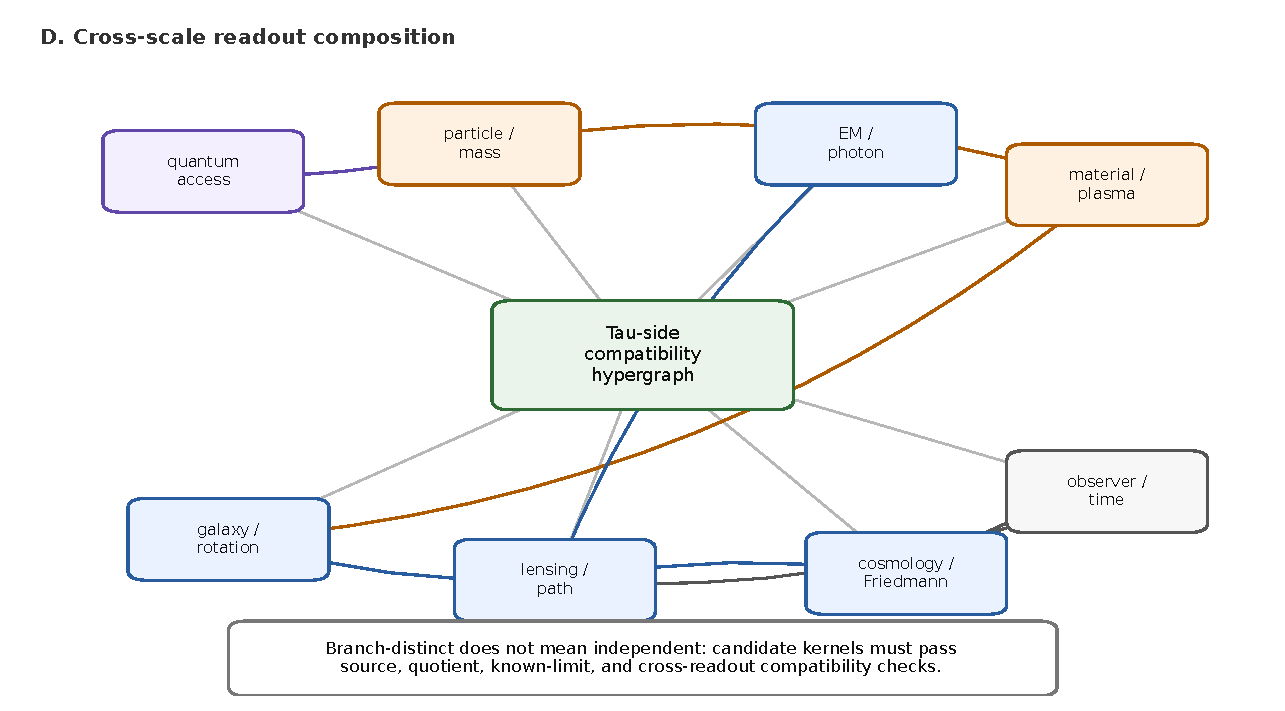
\includegraphics[width=0.95\linewidth]{figures/fig_cross_scale_readout_composition.pdf}
  \caption{Kereszt-skálájú readout-kompozíció.  A Tau Core readout-családjai
  ágszinten különbözők, de ez nem jelent operacionális függetlenséget.  A
  jelölt kerneleknek source-, carrier-, quotient- és cross-readout
  kompatibilitási feltételeket kell teljesíteniük, mielőtt scaffold státusz
  fölé emelhetők.  Az ábra architekturális: nem fizikai unifikációs bizonyítás.}
  \label{fig:cross-scale-readout-composition-hu}
\end{figure}

\begin{definition}[Relift]
Egy \(U_i\) kiolvasáshoz tartozó relift olyan térkép vagy részleges térkép
\[
  J_i:\Obs_i\to\RTspace,
\]
amely megpróbál parent-válasz reprezentánst rekonstruálni egy kiolvasott
rekordból.  Nem kell globálisan léteznie és nem kell egyértelműnek lennie.
\end{definition}

\begin{definition}[Kiolvasási obstrukció]
Ha \(r=\Rmap(s)\), akkor az elsődleges defektusobjektum nem vektorkivonás,
hanem obstrukciós rekord:
\[
  \omega_i(r)=0
  \quad\Longleftrightarrow\quad
  J_iU_i(r)\,N_i\,r.
  \label{eq:obstruction-hu}
\]
Vagyis nincs defektus, ha a relift ugyanabba a deklarált null-osztályba tér
vissza.  Csak affin vagy linearizált chartban reprezentálható ez a defektus
koordinátakülönbségként:
\[
  h_i(r)=J_i(U_i(r))-r.
  \label{eq:defect-hu}
\]
\end{definition}

Az obstrukciós feltétel és chart-szintű reprezentánsa nem sötétanyag-képlet és
nem kvantum-kollapszus képlet.  Absztrakt hiányossági rekord.  Egy fizikai
ágnak később meg kell adnia a kodomént, a quotientet, az egységeket, az ismert
limiteket és az empirikus tesztet.

\section{A primitív objektumok státusza}

Alapozó paper-ek gyakori hibája, hogy a definíció, feltételezés és levezetett
állítás összemosódik.  Az alábbi ledger ezért rögzíti az itt bevezetett
objektumok státuszát.  Ez nem plusz bizonyíték, hanem claim-boundary eszköz.

\begin{center}
\small
\textbf{Primitív objektumok státusz-ledgere}\\[0.5em]
\begin{tabular}{L{0.20\linewidth}L{0.30\linewidth}L{0.38\linewidth}}
\toprule
Objektum & Státusz ebben a paperben & Itt még nincs megadva\\
\midrule
\(\Ssrc\) & deklarált source/seed domén & minden forrás fizikai ontológiája\\
\(\RTspace\) & parent-választér, formai doménként feltételezve & egyediség vagy fizikai létezés bizonyítása\\
\(\Rmap\) & endpoint-vak válaszleképezés vagy reláció & dinamikai törvény vagy parent akció\\
\(\Mta\) & morfológia-kondicionáló test & első elvekből való levezetés\\
\(U_i^{\Mta}\) & szektor-readout definíció & kalibrált fizikai megfigyelhető modell\\
\(N_i\) & deklarált null/quotient politika & automatikus gauge-elv\\
\(J_i\) & opcionális relift eszköz & globális inverz readout\\
\(\omega_i\) & obstrukciós rekord \(N_i\) modulo & sötétszektor- vagy kollapszusmechanizmus\\
\bottomrule
\end{tabular}
\end{center}

A paper csak akkor válik nemtriviálissá, ha későbbi ágak a harmadik oszlop
elemeit source-oldali levezetésekkel, ismert-limit visszanyerésekkel vagy
bukott kontrollokkal váltják ki.  Addig ezek az objektumok fegyelmezett
nyelvet definiálnak, nem befejezett fizikai elméletet.

\section{Minimális kiolvasási kalkulus}

Az ebben a szakaszban használt matematika standard.  Egy readout partíciót
indukál a parent-választéren; a quotient-safety annak jól-definiáltsága a
megfelelő quotienten; a finomítás pedig a partíciók szokásos finomítási
rendje.  A Tau Core nem állít matematikai újdonságot ezekről a tényekről.
Könyvelési fegyelemként használja őket, hogy későbbi fizikai ágak ne rejtsenek
endpoint-szivárgást vagy double-countingot új terminológia mögé.  Ugyanez a
fogalmi terület érintkezik coarse-graining, marginalizáció, consistent-history,
decoherence-inspirált nyelvek és Jaynes-féle információelméleti statisztikus
mechanika irányaival \cite{Griffiths1984,GellMannHartle1990,Jaynes1957a,Jaynes1957b}.

Legyen \(\RTspace\) parent-választér és \(U_i\) kiolvasás.  Az első
matematikai objektum az indisztingválhatósági reláció:
\begin{equation}
  r\sim_i r' \quad\Longleftrightarrow\quad U_i(r)=U_i(r').
  \label{eq:readout-equivalence-hu}
\end{equation}
Ez readout-relatív.  Egy különbség lehet láthatatlan az egyik szektorban és
látható egy másikban.

\begin{definition}[Kiolvasási kernel]
\(U_i\) kiolvasási kernelje az \eqref{eq:readout-equivalence-hu} reláció.  Ha
\(\RTspace\) lineáris és \(U_i\) lineáris, ez a szokásos nulltérre
egyszerűsödik.  Általában azonban ekvivalenciareláció, nem feltétlenül
lineáris altér.
\end{definition}

\begin{definition}[Kiolvasási finomítás]
\(U_j\) finomítja \(U_i\)-t, ha
\[
  r\sim_j r'\Longrightarrow r\sim_i r'.
\]
Vagyis \(U_j\) legalább annyi parent-válasz információt különböztet meg, mint
\(U_i\).
\end{definition}

\begin{definition}[Közös kiolvasás]
\(U_i\) és \(U_j\) közös kiolvasása:
\[
  U_{ij}(r)=(U_i(r),U_j(r)).
\]
Ekvivalenciarelációja:
\[
  \sim_{ij}=\sim_i\cap\sim_j.
\]
\end{definition}

\begin{proposition}[A közös kiolvasás finomítja komponenseit]
\(U_{ij}\) finomítja \(U_i\)-t és \(U_j\)-t is.
\end{proposition}

\begin{proof}
Ha \(r\sim_{ij}r'\), akkor \(U_i(r)=U_i(r')\) és \(U_j(r)=U_j(r')\).  Tehát
\(r\sim_i r'\) és \(r\sim_j r'\).
\end{proof}

Ugyanez a nem-injektív kiolvasási gondolat később readout-medence
stabilitási elvként is megfogalmazható.  Egy deklarált \(R_{4D}\) kiolvasás
mellett egy stabil \(O\) objektumosztály medencéje:
\[
  \mathcal B_O=\{r\in\RTspace: R_{4D}(r)\simeq O\}.
\]
A \(\mathcal B_O\)-n belüli parent-válasz változás megőrzi a megfigyelt
objektumosztályt, míg egy látható átmenet vagy bomlás medenceátlépésként
olvasható.  Ez ebben a paperben csak objektum-tartóssági definíciós scaffold:
nem protonstabilitás-bizonyítás, nem Standard Modell-levezetés és nem
bomlási ráta képlet.

Ezért a több-kiolvasásos tesztek értékesek lehetnek, de ezt nem szabad
statisztikai függetlenséggel összekeverni.  Két readout lehet ugyanannak a
parentnek korrelált testvér-readoutja.  Minimális megfigyelési modell:
\[
  R_i=O_i[P]+N_i,
\]
ahol \(P\) közös látens parent, \(O_i\) a szektor readout-operátora, \(N_i\)
pedig zajt, szelekciót és pipeline-hatást gyűjt.  Kozmológiában például a
galaxis-klaszterezés, weak lensing, gáztracerek és CMB-lencsézés mind
ugyanarra az anyag/potenciál parentre reagálhatnak, miközben eltérő
megfigyelési operátorokat használnak.

Ezért a readoutok nyers egyezése önmagában nem Tau Core-jel.  Az erősebb kérdés
az, hogy marad-e közös residual a megfelelő null parentre való kondicionálás
után:
\[
  \Delta R_i=R_i-O_i[P_0].
\]
Kozmológiai ágban \(P_0\) lehet illesztett \(\Lambda\)CDM anyag/potenciál
parent; más ágban az adott standard baseline.  Tau Core-kompatibilis többlet
csak olyan residual cross-readout struktúra lehet, amely túléli a deklarált
nullmodellt, kovarianciát és source-overlap ledgert.  Ezt itt egyszerűen
source-overlap fegyelemnek nevezzük.  Ez nem validációs statisztika és nem
függetlenségi állítás.  E fegyelem nélkül a közös readout egyszerűen ugyanazt
a forráskoordinátát számolhatja kétszer.

Publikálatlan Tau Core protokolljegyzetek ugyanezt a fegyelmet konkrétabb
empirikus beállításokban is használják, de ezek a jegyzetek nem bizonyítékok
ehhez az alapozó paperhez.  Foundation Paper I ezért nem támaszkodik rájuk
eredményként; legfeljebb belső terminológiai provenance-ként kezeli őket.

\section{Nemtriviális reprezentációs feltétel}

A fenti nyelv önmagában túl általános.  Bármely megfigyelhető \(O\) triviálisan
beágyazható lenne úgy, hogy
\[
  \RTspace=\Obs,\qquad \Rmap(s)=O,\qquad U=\mathrm{id}_{\Obs}.
\]
Ez nem Tau Core magyarázat, hanem endpoint-átnevezés.

Ezért minden előléptetett ágnak teljesítenie kell egy nemtriviális
reprezentációs feltételt: a parent-választér, a válaszleképezés, a
morfológiai test, a null-politika és a readout nem redukálható veszteség nélkül
az endpoint identitás-readoutjára.  Legalább az alábbiak egyikét kell
parent-oldalról kikényszerítenie:
\begin{enumerate}[label=(N\arabic*)]
  \item quotient-safe null-struktúrát, amelyet az endpoint önmagában nem ad;
  \item több readout közötti közös forrás- vagy source-overlap relációt;
  \item ismert-limit visszanyerést;
  \item rossz családot, kontrollt vagy tiltott mentőutat kizáró szabályt;
  \item endpoint-vak módon fagyasztott numerikus értéket, relációt vagy null
  predikciót.
\end{enumerate}
Ha ez nem teljesül, az ág legfeljebb átírás, nem fizikai vagy matematikai
előrelépés.

Az ismert-limit visszanyerés önmagában nem elég.  Sok ártalmatlan átírás is
képes visszaadni egy már ismert limitet.  Előléptetéshez ezért legalább egy
endpoint-vak következmény is kell, amely elbukhatott volna: fagyasztott
numerikus érték, tiltott család, null predikció, source-oldali reláció vagy
kontroll-kizárás, mindez endpoint-inspekció előtt deklarálva.

\section{Nullok, quotientek és védett identitás}

Minden fizikai kiolvasásnak vannak null-irányaik: parent-változások, amelyeket
az adott readout fizikailag irrelevánsnak tekint.  Jelölje \(N_i\) a
null-relációt.  A quotient objektum:
\[
  [r]_i\in\RTspace/N_i.
\]
A kiolvasás quotient-safe, ha
\begin{equation}
  rN_i r'\Longrightarrow U_i(r)=U_i(r').
  \tag{QS-HU}
  \label{eq:quotient-safe-hu}
\end{equation}
Ha a \eqref{eq:quotient-safe-hu} quotient-safety feltétel sérül, a readout
különböző megfigyelhetőket rendel olyan parent
állapotokhoz, amelyeket maga fizikailag ekvivalensnek deklarált.

Ekvivalensen a readoutnak faktorizálnia kell a quotienten:
\[
  N_i\subseteq\sim_i,\qquad
  U_i=\bar U_i\circ q_i,\qquad
  q_i:\RTspace\to\RTspace/N_i.
\]
Itt \(\bar U_i\) a quotient-readout.  Ez formalizálja azt, hogy nullnak
nyilvánított parent-különbséget nem szabad fizikai megfigyelhetőként
visszaolvasni.

\begin{definition}[Védett forrásidentitás]
Védett forrásidentitás egy \(Q_{\rm src}\) ekvivalenciareláció a parent-oldali
forrásokon vagy forrásreprezentánsokon, amelyet a teória forrásszintű
identitásként kezel.  A readout source-faithful, ha nem omlaszt össze külön
\(Q_{\rm src}\)-osztályokat egy kiválasztott forrásosztályba anélkül, hogy ezt
védett null-szerkezetként deklarálná.
\end{definition}

Ez konzisztenciaigény.  Nélküle a modell tetszőleges különbségeket rejthet a
parent térbe, és csak az endpoint megtekintése után húzhatná elő őket.

\section{Endpoint-vakság mint tudományos szabály}

Endpoint-vak egy readout modell, ha a forrás, kernelcsalád, amplitúdószabály
és null-politika rögzítve van az endpoint residual megtekintése előtt.  Ez nem
filozófiai ízléskérdés.  Ez az egyetlen módja annak, hogy egy tág readout
keret ne váljon görbeillesztéssé.

A minimális endpoint-vak rekord tartalmazza:
\begin{enumerate}[label=(E\arabic*)]
  \item a forrásobjektumot vagy forrásproxyt;
  \item a deklarált \(U_i\) readout-családot;
  \item a null- és quotient-politikát;
  \item az együtt használt csatornák source-overlap döntését;
  \item freeze artifactot vagy időbélyegzett deklarációt;
  \item tiltott endpoint mezőket;
  \item kontrollokat és failure-feltételeket.
\end{enumerate}

Foundation Paper I nem futtat endpoint-tesztet.  Azt mondja ki, hogy a későbbi
ágaknak miért van rá szükségük.

\section{Hogyan jelenik meg effektív readout-változás?}

A Tau Core a primitív időfejlődést readout-paraméterezett változással váltja
ki.  Legyen \(r=\Rmap(s)\) parent-szinten időtlen.  Tegyük fel, hogy egy
\(U_i\) readout olyan rekordot ad, amely \(t_i\) paraméterrel koordinatizálható:
\[
  U_i(r)=o_i(t_i).
\]
Ekkor
\[
  \frac{do_i}{dt_i}
\]
a readouton belül értelmes.  Nem kell parent-idő szerinti deriváltnak lennie.
Ez a minimális értelem, amelyben ez a paper az ``effektív dinamika'' kifejezést
használja: readouton belüli paraméterezett változásként, nem levezetett fizikai
mozgásegyenletként.

Két readout ugyanarról a parent-válaszról eltérhet:
\[
  U_A(r)=o_A(t_A),\qquad U_B(r)=C_B.
\]
Az első időindexelt sorozatként, a második statikus korrelációként vagy
kényszerként szervezi ugyanazt a parent-választ.  Nincs ellentmondás.

\section{Toy modell effektív readout-idővel}

Legyen
\[
  r=(a_0,a_1,\ldots,a_n,c)\in\mathbb R^{n+2}.
\]
Definiáljuk:
\[
  U_{\rm seq}(r)=(a_0,a_1,\ldots,a_n).
\]
A \(k\) index effektív readout-idő koordinátaként választható, és véges differencia
írható:
\[
  \Delta a_k=a_{k+1}-a_k.
\]
A parent objektumban semmi nem fejlődött.  A parent-válasz már tartalmazta az
indexelt szerkezetet; a readout rendet adott neki.

Második readout:
\[
  U_{\rm sum}(r)=\sum_{k=0}^n a_k.
\]
Ez csak aggregátumot lát, idősort nem.  A rejtett komponens readout-relatív:
\(U_{\rm sum}\) számára elveszik a rendezési információ, míg \(U_{\rm seq}\)
számára például \(c\) marad rejtett.

Egy későbbi Tau Core time-readout modul egy kicsit gazdagabb véges toy modellt
is ad: az indexelt vektor helyett kis parent-morfológiai gráfot használ.
Jelölt eseménysorrendeket egyszerre lehet pontozni lokális szekvenciális
út-költséggel és globális parent-konzisztencia költséggel. Ebben a toyban a
lokális időtörténetként legtermészetesebb sorrend nem feltétlenül ugyanaz,
mint az a sorrend, amely a parent-affinitásokat a legjobban őrzi. Ez csak az
alapnyelvi állítást erősíti: sorrendérzékeny narratívákat nem kell
automatikusan jövőből múltba ható okságként olvasni. Toy szinten
értelmezhetők egy globálisan kötött parent-rekord különböző
időrend-readoutjaiként. Ebből nem következik fizikai óraelmélet,
retrokausalitás, Born-szabály vagy kvantumdinamika.

\begin{figure}[t]
  \centering
  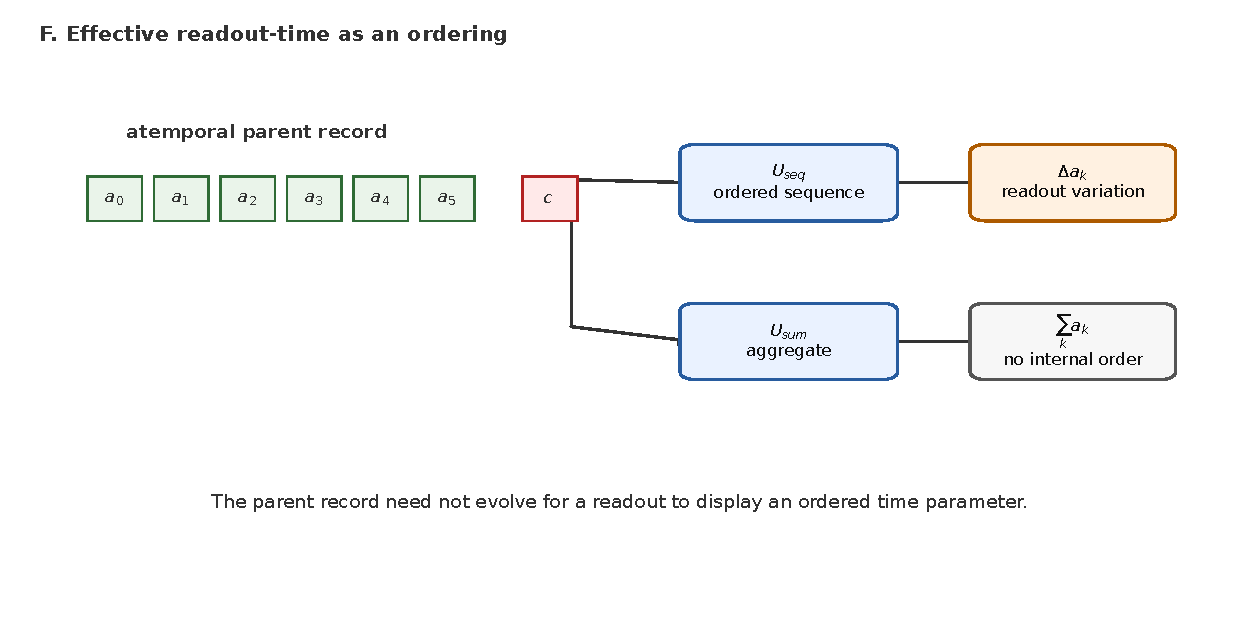
\includegraphics[width=0.95\linewidth]{figures/fig_effective_time_readout.pdf}
  \caption{Véges toy modell effektív readout-időre.  A parent rekord maga nem fejlődik.
  A sorozat-readout rendezett listát tár fel, ezért támogatja a \(\Delta a_k\)
  véges differenciákat.  Az aggregált readout más megfigyelhetőt ad, és elveszíti
  a belső sorrendet.}
  \label{fig:effective-time-hu}
\end{figure}

\begin{figure}[t]
  \centering
  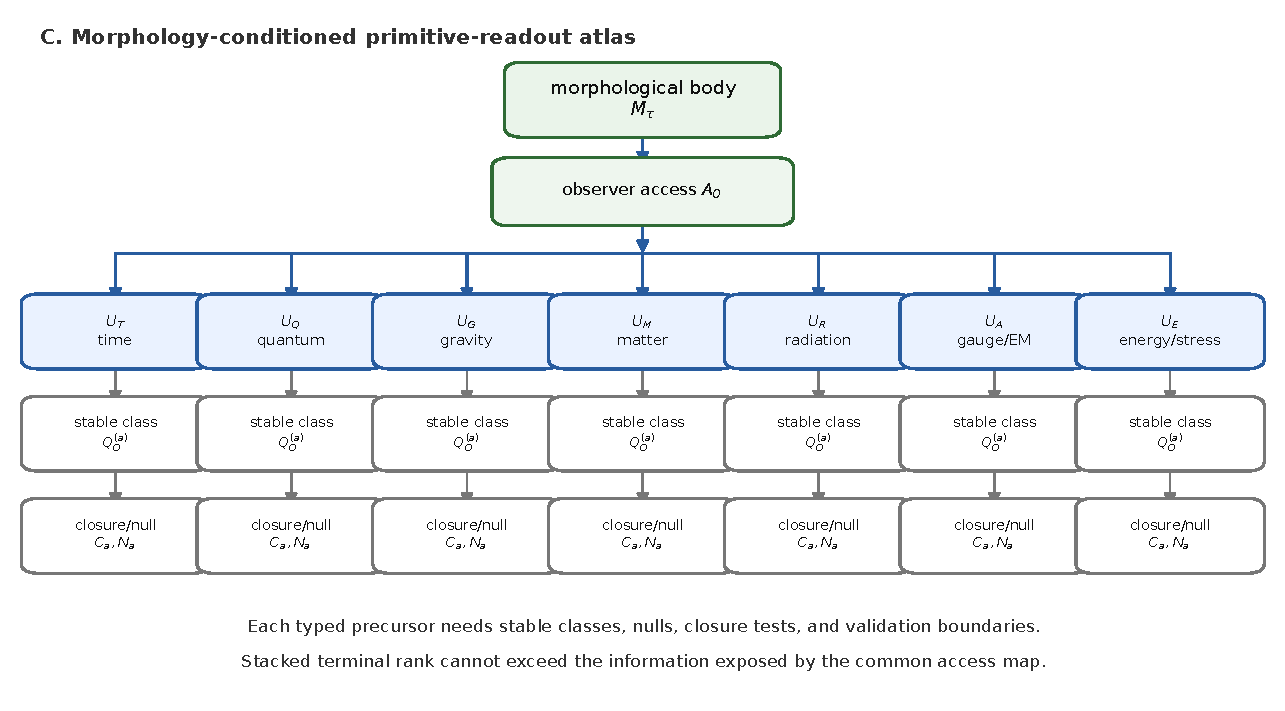
\includegraphics[width=0.95\linewidth]{figures/fig_readout_atlas.pdf}
  \caption{Egy parent-válasznak több szektor-kiolvasása lehet: téridő,
  megfigyelői idő, kvantum-hozzáférés, gravitációs válasz vagy tömeg/forrás
  struktúra.  Minden szektornak saját kodomén, null-politika, closure-teszt és
  validációs határ kell.}
  \label{fig:readout-atlas-hu}
\end{figure}

\section{Hét alapozó posztulátum}

Az alábbi posztulátumok nincsenek bizonyítva ebben a paperben.  A jelölt
keretet definiálják.

\begin{postulate}[Tau-szubsztrátum]
Létezik egy parent-szintű \(\T\) struktúra, amely az alapozó szinten nem
közönséges téridőbeli evolúció.
\end{postulate}

\begin{postulate}[Forrás-válasz]
A fizikai konfigurációkat parent-szinten endpoint-vak válaszok reprezentálják:
\[
  s\in\Ssrc,\qquad r=\Rmap(s)\in\RTspace.
\]
\end{postulate}

\begin{postulate}[Endpoint-vakság]
\(\Rmap(s)\), illetve bármely source objektum, amely readout-kernelt választ,
nem használhatja azt az endpoint residualt, amelyet később magyarázni akar.
\end{postulate}

\begin{postulate}[Readout-emergencia]
A megfigyelt fizikai leírások szektor-kiolvasások:
\[
  O_i=U_i^{\Mta}(\Rmap(s)).
\]
Az idő, téridő, kvantum-hozzáférés, gravitáció és tömeg/forrás leírás readout
jelölt, nem primitív kategória.
\end{postulate}

\begin{postulate}[Effektív readout-változás]
Időfejlődés csak akkor jelenik meg, ha egy readout stabil rendezést vagy
óra-koordinátát enged meg.  Egy \(\frac{d}{dt}U_i(\Rmap(s))\) derivált
effektív readout-derivált, nem primitív parent-idő derivált, és önmagában nem
fizikai mozgástörvény.
\end{postulate}

\begin{postulate}[Rejtett defektus]
Ha egy readout és megengedett reliftje nem állítja vissza a parent-válasz
reprezentánst a deklarált null-reláció modulo, tehát
\(\omega_i(r)\neq0\), az obstrukció a readout rejtett defektusaként kerül
rögzítésre.  A \(J_iU_i(r)-r\) különbség csak akkor használható
reprezentánsként, ha a választott chartban a kivonás értelmezett.
\end{postulate}

\begin{postulate}[Feszültség mint readout-kudarc]
Egyes megfigyelési vagy elméleti feszültségek modellezhetők readout-, closure-
vagy relift-defektusként.  Ez kutatási hipotézis, és csak source-frozen
szabályok, kontrollok, ismert limitek és holdout tesztek után válik fizikává.
\end{postulate}

\section{Az állítási létra}

A Tau Core egyik központi fegyelme az állítási szintek szétválasztása:
definíció, posztulátum, sejtés, feltételes tétel, toy modell, numerikus
evidencia és empirikus validáció nem felcserélhető.

\begin{figure}[t]
  \centering
  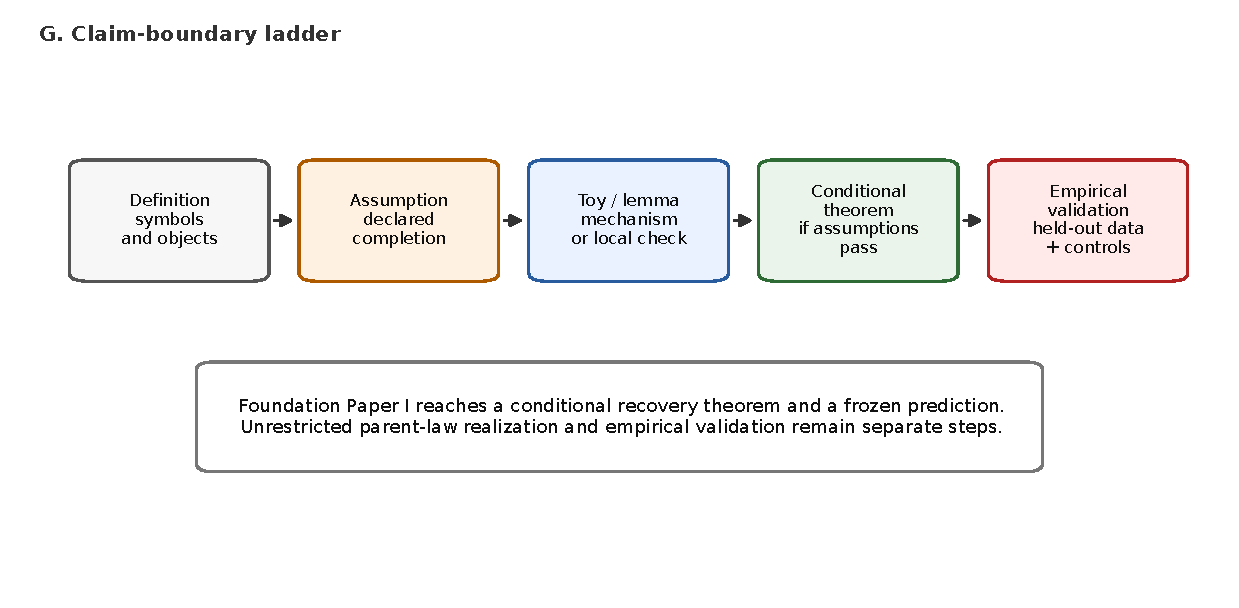
\includegraphics[width=0.95\linewidth]{figures/fig_claim_ladder.pdf}
  \caption{Foundation Paper I állítási létrája.  A kézirat definícióknál,
  posztulátumoknál, feltételes következményeknél és toy mechanizmusoknál áll
  meg.  Nem állít empirikus validációt.}
  \label{fig:claim-ladder-hu}
\end{figure}

A tág alapozó programok tipikus hibája a nyelvi előléptetés: metaforából
mechanizmus, mechanizmusból evidencia, evidenciából validáció lesz.  Ez a
paper ezt nem teszi.  Az, hogy az observer-time readout, nem vezet le fizikai
órát.  Az, hogy a sötét szektor esetleg hidden-defect nyelven is tárgyalható,
nem tünteti el a sötét anyagot.  Az, hogy a kvantumállapot readout lehet, nem
vezeti le a Hilbert-teret.

Egy későbbi Tau Core módszertani jegyzet, a Tau Core Readout Eligibility
Protocol v0.1 (TC-REP-0.1), ezt a fegyelmet pre-formális
readout-jogosultsági auditként rögzíti.  Azt kérdezi,
hogy egy jelölt ág kizárja-e a célontológiát a parent-feltevésekből,
nyilvántartja-e a primitív-adósságot, readout-mediáción keresztül halad-e,
kinyer-e valódi constraintet, landol-e matematikai és mérési oldalon,
elkülönül-e rivális magyarázatoktól, és megőrzi-e a bukási módokat.  Ez nem új
matematika és nem jelölés általi bizonyítás, hanem claim-boundary ellenőrző
lista arra, hogy egy ág több-e ismert fizika átnevezésénél.
A protokollnak van kompakt szimbolikus auditlánca is, de ez a paper
szándékosan a prózai ellenőrzőlistát használja, nem pedig levezetési
jelölésként kezeli a láncot.

\begin{figure}[t]
  \centering
  
\includegraphics[width=0.95\linewidth]{figures/fig_status_matrix.pdf}
  \caption{Foundation Paper I claim-status mátrixa.  A paper definiál és
  posztulál egy parent-válasz/readout architektúrát, valamint toy mechanizmust
  ad effektív readout-időre és rejtett defektusokra.  A narancs/piros elemek
  a non-claim státuszt jelölik: nincs empirikus validáció, nincs GR/QM/QFT
  vagy parent-akció deriváció.}
  \label{fig:status-matrix-hu}
\end{figure}

\section{Véges toy modell}

Legyen a parent-választér:
\[
  \RTspace=\mathbb R^3,\qquad r=(a,b,c).
\]
Két readout:
\[
  U_A(a,b,c)=(a,b),\qquad U_B(a,b,c)=(a,c).
\]
Ezek különböző koordinátákat felejtenek el.  Válasszunk kanonikus relifteket:
\[
  J_A(x,y)=(x,y,0),\qquad J_B(x,z)=(x,0,z).
\]
Mivel ez a toy válasz-tér lineáris, \(\RTspace=\mathbb R^3\), az obstrukció
koordinátakülönbségekkel reprezentálható.  Ez speciális toy-chart kényelem,
nem \(\omega_i\) általános definíciója.
Ekkor:
\[
  h_A(r)=J_AU_A(r)-r=(0,0,-c),
\]
és
\[
  h_B(r)=J_BU_B(r)-r=(0,-b,0).
\]
Ugyanannak a parent-válasznak tehát különböző readoutok alatt különböző rejtett
komponensei vannak.

\begin{proposition}[Readout-relatív rejtett komponens]
A fenti toy modellben ami \(U_A\) alatt rejtett, az \(U_B\) alatt látható
lehet, és fordítva.
\end{proposition}

\begin{proof}
\(c\) hiányzik \(U_A(a,b,c)\)-ből, és a \(J_A\) relift alatt
\((0,0,-c)\) defektusként jelenik meg.  Ugyanez a koordináta jelen van
\(U_B(a,b,c)\)-ben.  Hasonlóan \(b\) látható \(U_A\) alatt és rejtett \(U_B\)
alatt.
\end{proof}

A tanulság kicsi, de fontos.  Egy rejtett komponens nem szükségképpen új
szubsztancia.  Lehet olyan komponens, amelyet a választott readout nem tud
visszaemelni.  Hogy ennek van-e köze sötét szektorokhoz, kvantumméréshez vagy
gravitációhoz, az későbbi fizikai kérdés.  A toy modell csak a logikai
nyelvtant engedélyezi; nem kényszerít sötétszektor-, kvantum- vagy
gravitációs mechanizmust.

\paragraph{Quotient-safety a toy modellben.}
\(U_A\)-hoz a természetes null-reláció:
\[
  (a,b,c)\,N_A\,(a',b',c')
  \quad\Longleftrightarrow\quad
  a=a'\ \text{és}\ b=b'.
\]
Ekkor \(U_A\) quotient-safe, mert \(rN_A r'\) esetén:
\[
  U_A(r)=U_A(r').
\]
A \(c\) koordináta \(U_A\) számára láthatatlan, de ettől még nem új erő és
nem új szubsztancia.  Csak null-koordináta ebben a readoutban.  Ha ugyanazt a
readoutot később így módosítjuk:
\[
  U_A^{\rm bad}(a,b,c)=(a,b+\alpha c),
\]
miközben \(N_A\) marad a deklarált null-politika, quotient-safety sérül:
két \(N_A\)-ekvivalens parent reprezentáns különböző megfigyelhetőt adhat.
Ha egy ág fizikailag láthatóvá akarja tenni \(c\)-t, akkor a readoutot és a
null-politikát endpoint-inspekció előtt kell megváltoztatnia; nem használhat
csendben egy null-koordinátát endpoint-mentő korrekcióként.

\paragraph{Source-freeze a toy modellben.}
Tegyük fel, hogy egy ág source-szabályt javasol:
\[
  s=(a,b,c),\qquad c=f_{\rm src}(a,b;\theta),
\]
ahol \(f_{\rm src}\) és \(\theta\) source-oldali információból rögzített,
mielőtt bármilyen endpoint residualt megnéznénk.  Ekkor \(U_A(s)\), \(U_B(s)\)
és a megfelelő defektusok legitim toy-kimenetek a fagyasztott ágból.  Ha
viszont \(f_{\rm src}\), \(\theta\), vagy a \(c\) használatának döntése azért
születik, mert \(U_A\) elhibázott egy célértéket, akkor endpoint információ
szivárgott vissza a forrásdefinícióba.  Ez lehet fenomenológiai illesztés, de
nem Tau Core source-frozen deriváció.

\begin{figure}[t]
  \centering
  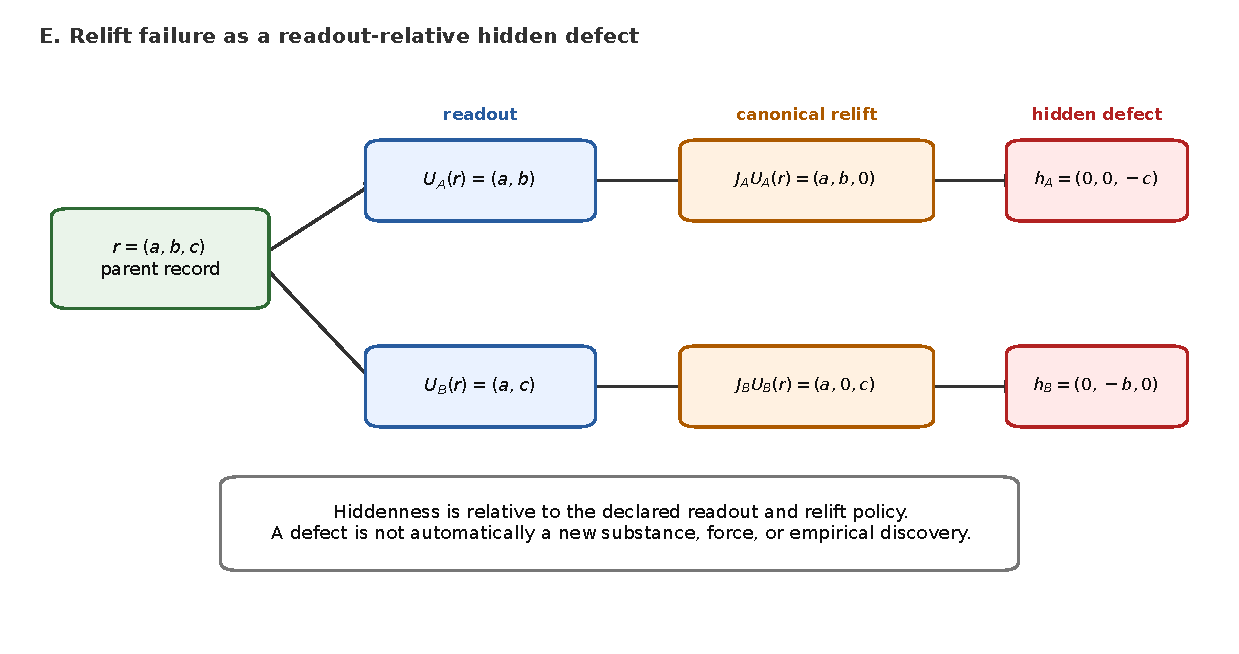
\includegraphics[width=0.95\linewidth]{figures/fig_hidden_defect.pdf}
  \caption{Readout-relatív rejtett defektusok.  Két kiolvasás ugyanarról a
  parent-válaszról különböző relift-kudarcot adhat.  A rejtett komponens
  először hiányossági rekord, nem automatikusan új erő vagy szubsztancia.}
  \label{fig:hidden-defect-hu}
\end{figure}

\section{Morfológiai test és vetített morfológia}

A ``morfológia'' szó félrevezető lehet.  Csillagászati használatban gyakran
látható alakot vagy katalógustípust jelent.  A Tau Core-ban az elsődleges
objektum nem a megfigyelt alak, hanem a Tau-oldali morfológiai test \(\Mta\).

A morfológiai test strukturált forrásobjektum, amely kiolvasásokat kondicionál.
Egy galaxis képe, rotációs görbéje, cosmic-web tenzora, lencsézési térképe vagy
kvantummérési kontextusa csak vetített handle lehet erre a testre.  Egyetlen
4D megjelenés gyakran nem tartalmaz elég információt a readout-releváns
forrásról: hiányozhat history, observer/path geometria, closure-osztály vagy
null-szerkezet.

Minimális forma:
\begin{equation}
  O_i=U_i^{\Mta}(\Rmap(s)).
  \label{eq:morph-conditioned-hu}
\end{equation}
A felső index azt jelzi, hogy a readout-térkép a morfológiai test által
kondicionált.  Ekvivalensen írható
\[
  U_i:\mathcal M_\tau\times\RTspace\to\Obs_i.
\]
Ez nem bizonyítja, hogy \(\Mta\) fizikailag le van vezetve; csak azt mondja,
hogy a readout-választás nem forrásmentes.

Konkrét ágban \(\Mta\)-nak admisszibilisnek és fagyasztottnak is kell lennie.
Ez azt jelenti, hogy a \(\Mta\)-t kiválasztó vetített handle-öket, a megengedett
readout-kernelcsaládot és a csatornák közötti source-overlap döntéseket
endpoint scoring előtt deklarálni kell.  Ha \(\Mta\) az endpoint residual
megtekintése után változik, az ág phenomenological-only státuszú marad, hacsak
független forrásreview nem nyitja újra a választást.

\section{Megfigyelői idő}

A Tau Core a megfigyelői időt readoutként kezeli, nem parent-oldali primitív
paraméterként:
\begin{equation}
  t_{\rm obs}^{S}
  =
  U_{\rm time}^{S}(\Rmap(s),\Mta,\mathcal O_S,\gamma_S),
  \label{eq:observer-time-hu}
\end{equation}
ahol \(S\) szektor, \(\mathcal O_S\) megfigyelői interface-adat, \(\gamma_S\)
pedig útvonal- vagy szelvényadat.

Ez nem levezetett óraelmélet, hanem fegyelmi szabály.  Azt mondja, hogy a
megfigyelő ideje a megfigyelő readout-csomagjához tartozik.  Egy későbbi
fizikai elméletnek kell megmutatnia, mikor redukálódik sajátidőre és mikor
enged korrekciókat.

\section{Kvantum-readout}

A kvantumág természetes célpontja a readout-nyelvnek, de itt különösen veszélyes
a túlállítás.  Minimálisan:
\begin{equation}
  q=U_q(\Rmap(s)),
\end{equation}
ahol \(q\) hozzáférési állapot vagy valószínűségi hozzárendelés rekordja lehet.
Ez messze van a Hilbert-tér vagy Born-szabály levezetésétől.

A kvantumrekonstrukciós programok megmutatják, hogy a kvantumelmélet
információelméleti vagy operacionális axiómákból is közelíthető
\cite{Hardy2001,Chiribella2011,MasanesMueller2011}.  A generalizált
probabilisztikus és Jordan-algebrai utak azt is mutatják, mennyi struktúra kell
ahhoz, hogy Hilbert-tér jellegű kvantumelmélet kényszerüljön
\cite{BarnumWilce2014}.  A Tau Core ezeket boundary-discipline-ként használhatja,
de nem állíthatja, hogy pusztán egy véges kontextuális readout-grammar már
komplex Hilbert-teret implikál.

\begin{quote}
Ha a Tau Core rendezett konvex hozzáférésiállapot-teret, szeparáló effektusokat,
megfelelő ön-dualizáló párosítást, folytonos homogén reverzibilis szimmetriát,
kompozíciós merevséget és trace-egyértelműséget szolgáltat, akkor a
Born/Hilbert-reprezentáció feltételes célponttá válik.
\end{quote}
Ez a lista orientáció, nem rejtett kvantummechanika-import.  A konvex állapotok
és szeparáló effektusok a preparáció/mérés elválasztását rögzítik; a
szimmetria-, kompozíciós és trace-feltételek olyan regularitások, amelyek a
Hilbert-szerű kvantumelméletet megkülönböztetik egy általános valószínűségi
kalkulustól.  A Tau Core-nak egy későbbi kvantumágban ezeket is le kellene
vezetnie vagy függetlenül igazolnia.
Az itt felsorolt feltételek nem a Foundation Paper I posztulátumai.  Példák
arra az extra rekonstrukciós struktúrára, amelyet egy későbbi kvantumágnak
szállítania vagy helyettesítenie kellene.

Egy lehetséges későbbi worked branch egy véges fázisragasztási toy modell
lehetne.  Ebben egy branch deklarálna source-frozen primitív frame-et,
kiválasztott párokon fázis- vagy kontextuskapcsolatot, reverzibilis rank-2
kontrasztmozgásokat, invariáns trace/effektus párosítást és közös null
policyt.  Ha a kiválasztott hármasokon a ciklikus fázisösszeg eltűnne, akkor
a páronkénti fázisadatok globális komplex fázischarttá ragaszthatók lennének.
Ez az ordinary mathematics of gluing local phase data irányába mutatna, nem
önmagában Tau Core bizonyításra.  Foundation Paper I ezért nem állít
Hilbert/Born recoveryt.  Egy ilyen későbbi kvantumágnak külön appendixben vagy
tételszakaszban kellene rögzítenie minden finite-domain, frame, trace,
null-policy és source-freeze feltételt, mielőtt a
\(p(E|\rho)=\mathrm{Tr}(\rho E)\) alak akár toy-szinten is állítható lenne.

Ebben a korlátozott értelemben a kvantum-readout nem zárt sziget.  Egy
parent-oldali különbség, amely hozzáférési, fázis-, kontextuális vagy nem
kommutáló szerkezetet hordoz, rendelkezhet kvantum-facing és nem-kvantum-facing
vetületekkel is.  Ha ez a különbség túléli egy gravitációs, tömeg/forrás,
megfigyelői idő vagy kozmológiai readout null-quotientjét, akkor quantum-like
nyom megjelenhet az adott szektor residual-szerkezetében.  Ez nem azt állítja,
hogy a kvantummechanika közvetlenül hat minden más readoutra.  Csak azt az
óvatosabb állítást teszi, hogy több readout ugyanannak a parent-oldali
szerkezetnek különböző aspektusait teheti láthatóvá, és ezt source-overlap és
double-counting szabályokkal kell kontrollálni.

\section{Gravitációs és sötétszektor-readoutok}

A gravitációs ág motiválja a hidden-defect szókészletet.  Egy gravitációs
kiolvasás nem biztos, hogy minden forrásreleváns struktúrát vissza tud emelni
Newtoni, relativisztikus vagy closure-kompatibilis leírásba:
\begin{equation}
  \omega_g(r)=0
  \quad\Longleftrightarrow\quad
  J_gU_g(r)\,N_g\,r,
  \qquad r=\Rmap(s).
\end{equation}
Ha \(\omega_g(r)\neq0\), és az obstrukciós rekord túléli a deklarált null
quotientet mérhető 4D readouttal, akkor residual-csatorna jelölt.  A
\[
  h_g=J_gU_g(r)-r
\]
koordinátakülönbség csak akkor használható, ha már választottunk olyan
linearizált gravitációs chartot, amelyben a kivonás értelmezett.  Ez még nem
sötétanyag-helyettesítés.

\section{Kozmológiai readout}

A kozmológia természetes readout célpont, mert az expanziós történet,
távolságlétra, növekedési adatok, lencsézés és CMB-inferencia mind
modellfüggő readout-feltételezéseken keresztül tömörülnek.  Sémában:
\begin{equation}
  O_{\rm cosmo}
  =
  U_{\rm cosmo}(\Rmap(s),\Mta^U,\gamma_{\rm path},\mathcal O_{\rm obs}).
\end{equation}
Itt \(\Mta^U\) univerzumléptékű morfológiai test, \(\gamma_{\rm path}\)
útvonal/környezet adat, \(\mathcal O_{\rm obs}\) pedig megfigyelői interface.
Ez nem eredmény, hanem figyelmeztetés: a kozmológiai feszültségeket nem szabad
egyetlen skálafaktor-függvénybe összenyomni explicit forrás- és kovarianciafegyelem
nélkül.

\section{Viszony a meglévő papersorozathoz}

Az arab számozású Tau Core paperek nem szükségesek e foundation paper logikájához.
Szűkebb, operacionális csomagok: galaxis-residualok, source-frozen morfológia
vagy projekciós kernelek, sötétszektor-döntési protokollok, kozmológiai vagy
web-witness auditok.  Ezek nem bizonyítják a parent ontológiát.

Foundation Paper I ezzel szemben a közös szókészletet rögzíti.  Nem kölcsönzi
a numerikus eredményeket bizonyítékként.  Egy későbbi pozitív audit motiválhatja
a keretet, de nem validálja a parent elméletet, ha a parent forrástól a readout
szabályig vezető út nem fagyasztott, nem körkörös és nem tesztelt.

\section{Viszony MOND-hoz és sötét anyaghoz}

A Tau Core-t nem érdemes anti-MOND vagy anti-dark-matter keretként bemutatni.
Pontosabb és védhetőbb pozíció az, hogy harmadik szintű nyelvet próbál adni:
olyan readout-nyelvet, amelyben a MOND-szerű fenomenológia és a
sötétanyag-szerű jelek is lehetnek mélyebb forrásstruktúra effektív
kiolvasásai.

A MOND-program számára vonzó pont, hogy a Tau Core nem abból indul ki, hogy a
standard hideg részecskehalo-kép biztosan a teljes történet.  Megengedi, hogy
a galaxisléptékű gyorsulási regularitások mélyebb gravitációs/readout
struktúrából következzenek.  Ugyanakkor a Tau Core nem lépteti elő magát a
MOND-ot végső ontológiává.  A MOND-szerű törvényeket, ha megjelennek,
köztes effektív szabályként kezeli:
\[
  \text{MOND-szerű regularitás}
  \quad\leadsto\quad
  \text{egy mélyebb morfológia effektív readout-limitje}.
\]
Ez ebben a paperben nem MOND-levezetés.  Claim-boundary állítás: a Tau Core
megpróbálhatja megérteni, miért jelenik meg MOND-szerű skála vagy reláció, de
ehhez a skálát le kell vezetnie, vissza kell adnia az ismert limiteket, és
kontrollokon kell átmennie.

A sötétanyag-program felé más az óvatosság.  A Tau Core-nak nem szabad túl
korán azt mondania, hogy a sötét anyag puszta illúzió.  A lencsézés, CMB, BAO,
halmazadatok és struktúranövekedés a standard kozmológiai inferenciában erős
többletgravitációs szerkezetre mutatnak.  Egy Tau Core ágnak inkább ezt a
felbontott kérdést kell feltennie:
\[
  \begin{aligned}
  \text{sötétszektor-jel}
  \sim{}&
  \text{gravitáló tartalom}
  + \text{barionos maradványok}\\
  &+ \text{módosult válasz}
  + \text{readout/útvonal/morfológiai effektusok},
  \end{aligned}
\]
ahol ez séma, nem kész modellegyenlet.  A tudományos feladat az, hogy melyik
komponens melyik readout-csatornában van jelen, és van-e olyan komponens,
amely valóban ütközésmentes anyagként viselkedik.

Ezért a legjobb nyilvános framing:
\begin{quote}
A Tau Core nem anti-MOND és nem anti-dark-matter.  Readout-szintű formai nyelv,
amelyben a MOND-szerű gyorsulási törvények, a sötétanyag-szerű
lencsézési/kozmológiai jelek és a megfigyelőfüggő residualok source-frozen
komponensekre bonthatók és egymás ellen tesztelhetők.
\end{quote}
Ez nem győzelmi narratíva.  Nem azt mondja, hogy a meglévő táborok egyszerűen
tévedtek.  Azt mondja, hogy különböző táborok ugyanannak a mélyebb problémának
különböző vetületeit láthatták, és a hasznos kérdés az, hogyan lehet ezeket a
vetületeket endpoint leakage nélkül szétválasztani.

\section{Összevetés közeli gondolatokkal}

\paragraph{Relációs idő.}
A relációs idő megközelítései megmutatják, hogyan nyerhető dinamika
korrelációkból.  A Tau Core egyetért azzal, hogy külső idő nem feltétlenül
primitív, de ezt szélesebb readout-atlaszba helyezi.

\paragraph{Shape dynamics és relációs konfiguráció.}
A shape-dynamics inspirált munka arra figyelmeztet, hogy a téridő-struktúra
más szimmetria- vagy relációs választással is reformulálható
\cite{GomesKoslowski2012}.  A Tau Core ezt analógiaként használja, nem
bizonyításként.

\paragraph{Kvantumrekonstrukció.}
A kvantumrekonstrukciós programok mintát adnak arra, hogyan lehet operacionális
elvekből formalizmust építeni.  A Tau Core kvantumágának hasonló szintet kell
elérnie.

\paragraph{Holográfia és hibajavítás.}
A holografikus kvantumhibajavítás megmutatja, hogy bulk-szerű struktúra
nemtriviálisan kódolható és rekonstruálható határadatból
\cite{AlmheiriDongHarlow2015}.  Itt ez readout/rekonstrukciós fegyelem analógiája,
nem Tau-ontológiai bizonyíték.

\section{Mi számítana előrelépésnek?}

A keret akkor erősödik, ha az absztrakt readout-nyelv korlátos feladatokká
válik:
\begin{enumerate}[label=(\arabic*)]
  \item nem körkörös parent válaszlaw \(\Rmap\) levezetése;
  \item source-realizable morfológiai test \(\Mta\) definiálása;
  \item quotient-safe null-politika bizonyítása egy readoutnál;
  \item ismert fizikai limit, például sajátidő vagy Newtoni gravitáció
  kontrollált readout-limitként való levezetése;
  \item source-frozen empirikus szabályok, amelyek holdout teszten túlélnek;
  \item negatív eredmények megőrzése a bukott kernelek utólagos újrahangolása
  helyett.
\end{enumerate}

A ``parent válaszlaw'' kifejezést ez az alapozó paper szándékosan nem köti
egyetlen matematikai típushoz.  Lehetséges típusok:
\[
\begin{array}{ll}
\text{variációs törvény} & \Rmap \text{ akcióból vagy extremális elvből választódik ki},\\
\text{kényszertörvény} & \Rmap \text{ admisszibilitási vagy closure-egyenletekből jön},\\
\text{algebrai closure} & \Rmap \text{ source/readout konzisztenciából rögzül},\\
\text{probabilisztikus kernel} & \Rmap \text{ endpoint-vak átmeneti kernel},\\
\text{fixpont} & \Rmap \text{ válaszoperátor stabil megoldása},\\
\text{funktoriális szabály} & \Rmap \text{ struktúramegőrző source-térképekből indukált}.
\end{array}
\]
Itt egyik út sincs kiválasztva.  Egy későbbi ágnak előre deklarálnia kell,
melyik típust használja, mielőtt fizikai törvény levezetését állítaná.

Ez az alapozó réteg legnagyobb megmaradt gyengesége.  Az absztrakt
\(\Rmap\) jel csak könyvelés, amíg legalább egy ág nem rögzíti a matematikai
típusát, és nem visz végig egy láncot:
\[
  \text{forrás}\to\Rmap\to U_i^{\Mta}
  \to \text{ismert limit vagy fagyasztott, cáfolható következmény}
\]
endpoint leakage nélkül.  Foundation Paper I szándékosan megáll e választás
előtt; egy későbbi worked branch már nem állhat meg itt.

\section{Mi számítana bukásnak?}

Egy reviewernek nem kellene kitalálnia a bukási feltételeket.  Foundation
szinten a Tau Core gyengülne vagy visszaminősülne, ha a következők tartósan
fennállnak:
\begin{enumerate}[label=(F\arabic*)]
  \item \textbf{Nincs source-realizable parent objektum.}  Ha egy ághoz nem
  adható nem körkörös parent-oldali forrásosztály, az ág szókészlet marad,
  nem fizika.
  \item \textbf{Nincs quotient-safe readout.}  Ha deklaráltan null-ekvivalens
  parent reprezentánsok különböző megfigyelhetőket adnak, a readout belsőleg
  inkonzisztens.
  \item \textbf{Nincs ismert-limit visszanyerés.}  Ha egy ág nem tudja
  visszaadni a releváns standard limitet -- például sajátidőt, Newtoni
  gravitációt, Born-valószínűségeket vagy \(\Lambda\)CDM viselkedést --, nem
  léptethető elő.
  \item \textbf{Endpoint leakage.}  Ha a forrásosztály, kernelcsalád vagy
  amplitúdószabály abból a residualból van kiválasztva, amelyet később magyaráz,
  az illesztés, nem Tau Core deriváció.
  \item \textbf{Kontrollálatlan mentés.}  Ha minden bukás utólag hozzáadott,
  nem korlátozott projekciós csatornával javítható, a keret elveszíti
  tudományos tartalmát.
\end{enumerate}

Ezek nem puszta módszertani preferenciák.  Ezek azok a feltételek, amelyek
alatt az alapnyelv nem válik fizikai kutatási programmá.  A negatív eredményt
valódi visszaminősítésként kell megőrizni, nem terminológiai váltással elrejteni.

Az elfogadott visszaminősítési státuszok szigorú jelentése:
\begin{center}
\small
\begin{tabular}{L{0.28\linewidth}L{0.60\linewidth}}
\toprule
Státusz & Szigorú jelentés\\
\midrule
\textsc{toy-only} & nincs fizikai kodomén, egység vagy operacionális megfigyelhető\\
\textsc{phenomenological-only} & ismert adatot rendez vagy illeszt, de nincs parent-source deriváció\\
\textsc{blocked} & hiányzik ismert-limit, quotient-safety vagy source-realizability\\
\textsc{rejected} & fagyasztott predikció bukik holdouton/kontrollon, vagy leakage van\\
\bottomrule
\end{tabular}
\end{center}
Tiltott mentőműveletek: endpoint utáni kernelcsere, residualból választott
morfológiai paraméter, utólag beillesztett path/projection faktor, illetve a
kovariancia- vagy null-politika endpoint-inspekció utáni átírása.  Egy
előléptetett ágnak legalább egy fagyasztott numerikus értéket, relációt,
kizárást vagy null predikciót kell adnia az endpoint megtekintése előtt.

\paragraph{Minimális bukott ág példa.}
Legyen egy toy ágban a deklarált null-politika \(n\sim n'\), és a readout:
\[
  R(x,n)=x.
\]
Ha az ág később egy \(A\,n\) korrekciót ad hozzá egy endpoint residual
magyarázatára, akkor deklarált null-koordinátát használt fizikai
megfigyelhetőként.  Ez quotient-safety bukás.  Ha \(A\)-t vagy az
\(n\)-függés alakját az endpoint residual megtekintése után választotta, akkor
endpoint-vakságot is sért.  Ez nem Tau Core deriváció: \textsc{rejected}
státuszba kerül, vagy endpoint nélküli esetben legfeljebb
\textsc{phenomenological-only}.  A példa direkt triviális: azt mutatja, hogy
a keret egzotikus fizika nélkül is tud nemet mondani.

\section{Várható ellenvetések}

\paragraph{Ez csak nyelvváltás.}
Komoly ellenvetés.  A keret csak akkor hasznos, ha a readout-nyelv új
kényszereket kényszerít ki: endpoint-vakságot, null/quotient safety-t,
source-overlap fegyelmet, ismert-limit visszanyerést és explicit
failure-feltételeket.

\paragraph{A parent-válasz nem megfigyelhető.}
Feltételezés szerint nem közvetlenül megfigyelhető.  Ez önmagában nem végzetes:
sok elméleti objektum csak korlátozott hatásokon keresztül inferált.  A kérdés
az, hogy a deklarált readout-szabály ad-e olyan előrejelzést vagy kizárást,
amely bukhatott volna.

\paragraph{A keret bármit megmagyaráz.}
Ez a legfontosabb veszély.  Ezért kell megőrizni a negatív eredményeket.  Egy
bukott fagyasztott kernel visszaminősítendő, nem újrahangolandó.

\paragraph{Az időtlen válasz blokk-univerzumnak hangzik.}
A különbség az \eqref{eq:block-readout-hu} egyenlet: a 4D blokk itt readout,
nem végső ontológia.

\paragraph{Nincs fizikai törvény levezetve.}
Helyes.  Foundation Paper I nem vezet le fizikai törvényt.  Azokat az
objektumokat definiálja, amelyekre egy későbbi levezetésnek szüksége lenne.

\section{Strukturális predikciók, nem anomália-korrekciók}

Az ontológiai kérdés az, hogy a Tau Core nyelve tud-e olyan predikciót adni,
amely nem pusztán egy meglévő keret -- például MOND, \(\Lambda\)CDM, GR vagy
kvantumelmélet -- anomáliájára adott korrekció.  Foundation Paper I válasza
feltételes.

Egy Tau Core predikció nem attól strukturálisan eredeti, hogy residual tagot
ad egy baseline-egyenlethez.  Csak akkor számítana annak, ha egy
source-frozen parent/morfológiai szabály endpoint-inspekció előtt kényszerít
ki valamit.  Sematikusan:
\[
  \mathrm{Struct}_{\tau}(s,\Mta)=0
  \quad\Longrightarrow\quad
  \mathrm{Constraint}(U_i^{\Mta},U_j^{\Mta},N_i,N_j),
\]
vagy kizárásként:
\[
  \mathrm{Struct}_{\tau}(s,\Mta)
  \quad\Longrightarrow\quad
  \text{a }P\text{ readout-minta inadmisszibilis}.
\]
Ilyen típusú kényszer lehet:
\begin{itemize}
  \item kompatibilitási feltétel, amely két readout együttmozgását kényszeríti;
  \item null/quotient szabály, amely egy látszólagos korrekciót double-counting
  miatt kizár;
  \item medence-átmeneti invariáns, amely korlátozza, mely readout-átmenetek
  jelenhetnek meg stabil 4D eseményként;
  \item rank-, kapcsoltsági vagy frame-gluing feltétel, amelynek teljesülnie
  kell Hilbert-szerű vagy metrikus reprezentáció előtt;
  \item fagyasztott source-szabály, amely holdout csatornában hiányzó, tiltott
  vagy korrelált jellemzőt jósol.
\end{itemize}

Ez csak akkor Tau Core-specifikus predikció, ha a parent forrásból, a
morfológiai testből, a null-politikából és a readout-kompatibilitási szabályból
van rögzítve endpoint-inspekció előtt.  Ha ugyanaz a struktúra azért kerül be,
mert egy ismert baseline residualt hagy, akkor anomália-motivált korrekció,
nem parent-morfológiai predikció.  Ez a paper a kritériumot adja meg; validált
fizikai példát még nem.

\paragraph{Konkrét kizárás framework-szinten.}
A keret egy nemtriviális modellezési lépést már ezen a szinten is tilt.
Tegyük fel, hogy két szektor-korrekció alakja:
\[
  \Delta O_i=A_i\,q,\qquad \Delta O_j=A_j\,q,
\]
ahol \(q\) ugyanaz a source-oldali koordináta vagy proxy.  Ha az ág endpoint
inspekció előtt nem deklarál source-oldali felbontást \(q=(q_i,q_j)\),
ortogonalitási/kovariancia szabályt, vagy shared-parent kovarianciamodellt,
akkor a két tag nem kezelhető független evidenciaként és nem adható hozzá
független korrekcióként.  Ugyanazt a source szabadsági fokot olvasná ki
kétszer.  Így a Tau Core tiltja a ``same-source double counting'' használatát
admisszibilis magyarázatként.  Ez nem új fizikai predikció, de strukturális
kizárás, amely túlmegy a puszta átnevezésen.

\section{Minimális matematikai érettségi checklist}

\begin{center}
\begin{tabular}{p{0.28\linewidth}p{0.58\linewidth}}
\toprule
Követelmény & Jelentés\\
\midrule
Forrásdeklaráció & A parent-oldali forrás vagy proxy endpoint scoring előtt deklarált.\\
Readout kodomén & Az \(\Obs_i\) megfigyelhető tér specifikált.\\
Null-politika & Gauge, redundancia és protected-null irányok deklaráltak.\\
Quotient safety & Ekvivalens parent reprezentánsok azonos readoutot adnak.\\
Relift-politika & Az ág kimondja, hogy \(J_i\) létezik-e és hogyan.\\
Ismert limit & A readout visszaad standard limitet, ahol kell.\\
Failure-szabály & Bukott kontroll demóciót okoz, nem utólagos retuningot.\\
\bottomrule
\end{tabular}
\end{center}

Ez gyengébb, mint egy teljes fizikai elmélet, de erősebb, mint egy metafora.

\section{A római alapozó sorozat}

Ez a paper külön római számozású foundation sorozat első tagja:
\[
\begin{array}{ll}
\text{Paper 1--18} & \text{korlátos empirikus vagy protokoll-csomagok},\\
\text{Foundation Paper I, II, ...} & \text{fogalmi és matematikai alapozó paperek}.
\end{array}
\]

Javasolt következő tagok:
\begin{itemize}
  \item \textbf{Foundation Paper I}: időtlen morfológiai readout, fizikai
  validációs claim nélkül.
  \item \textbf{Foundation Paper II: A Finite Readout-Time Branch}: worked
  branch forrásdeklarációtól effektív readout-idő sorrendig, ismert-limittel
  vagy fagyasztott failure-szabállyal.
  \item \textbf{Foundation Paper III}: kvantum-readout, feltétlen Hilbert-,
  Born- vagy QFT-levezetés nélkül.
  \item \textbf{Foundation Paper IV}: hidden defects és sötét szektorok,
  sötétanyag- vagy sötétenergia-helyettesítési claim nélkül.
  \item \textbf{Foundation Paper V}: observer-time és kozmológia, Hubble
  tension vagy \(\Lambda\)CDM replacement claim nélkül.
  \item \textbf{Foundation Paper VI}: flavor és neutrino readout, Standard
  Model vagy neutrino-anomaly claim nélkül.
\end{itemize}
A következő foundation kéziratnak nem pusztán újabb általános framework-réteget
kell hozzáadnia.  Legalább egy worked branch-et kell tartalmaznia:
\[
  \text{forrás}\to \Rmap \to U_i^{\Mta}
  \to
  \text{ismert limit vagy fagyasztott, cáfolható következmény}.
\]

\section{Kompakt formai összegzés}

A keret objektumcsomagként:
\[
  \mathfrak T
  =
  (\Ssrc,\RTspace,\Rmap,\Mta,\{U_i\},\{N_i\},\{J_i\}).
\]
Itt \(\Ssrc\) forrásdomén, \(\RTspace\) válaszdomén, \(\Rmap\)
endpoint-vak válaszreláció, \(\Mta\) morfológiai test, \(U_i\) readout,
\(N_i\) null-politika, \(J_i\) opcionális relift.

Minimális konzisztenciafeltételek:
\begin{align}
  &s \text{ endpoint leakage nélkül rögzített},\\
  &r=\Rmap(s) \text{ definiált a deklarált forrásdoménen},\\
  &rN_i r'\Rightarrow U_i(r)=U_i(r'),\\
  &\omega_i(r)=0 \Longleftrightarrow J_iU_i(r)N_i r,\\
  &h_i(r)=J_iU_i(r)-r \text{ csak chart-szintű reprezentáns, ha értelmezett},\\
  &\text{ismert fizikai limitek visszanyerése előléptetés előtt}.
\end{align}

A paper legerősebb állítása az, hogy \(\mathfrak T\) belsőleg szervezett
kiinduló csomag readout-alapú kutatási programhoz.  Ez nem formális
konzisztenciabizonyítás minden lehetséges Tau Core ágra, és nem bizonyítja,
hogy a természet ilyen csomagot használ.

\section{Mit nem bizonyít a paper?}

\begin{itemize}
  \item Nem bizonyítja, hogy a Tau-szubsztrátum fizikailag létezik.
  \item Nem ad parent akciót.
  \item Nem vezeti le a fizikai időt.
  \item Nem vezeti le az általános relativitáselméletet.
  \item Nem vezeti le a kvantummechanikát, Born-szabályt, kollapszust vagy QFT-t.
  \item Nem vezeti le a Standard Modellt.
  \item Nem magyarázza meg a neutrínófizikát.
  \item Nem tünteti el a sötét anyagot vagy sötét energiát.
  \item Nem validál empirikus Tau Core claimet.
\end{itemize}

Ezek a korlátok nem lábjegyzetek.  A claim részei.  Az alapozó paper célja,
hogy a blokkolókat elég láthatóvá tegye ahhoz, hogy későbbi munka egyenként
támadhassa őket.

\section{Konklúzió}

A Tau Core itt időtlen morfológiai readout keretként jelenik meg.  Az alapjavaslat:
\[
  s\mapsto\Rmap(s)\mapsto U_i^{\Mta}(\Rmap(s)).
\]
Ebben az olvasatban a 4D téridőblokk nem végső ontológia, hanem egy readout:
\[
  M_{4D}=U_{4D}^{\Mta}(\Rmap(s)).
\]
A fizikai idő ugyanígy readout-csatorna, nem maga a \(\tau\) jelentése.

A paper hozzájárulása nem új empirikus eredmény, hanem korlátos szókészlet:
parent forrásmag, endpoint-vak válasz, morfológiai test, szektor-readout,
relift, rejtett defektus, observer-time readout és állítási létra.  Ez a
szókészlet későbbi munkának élesebb kérdéseket ad: mely readoutok
source-realizable-ek, mely defektusok élik túl a quotientet, mely ismert
limitek nyerhetők vissza, mely source-frozen kernelek élik túl a holdout
adatokat, és mely ágak buknak el.

A legtisztább összegzés:
\begin{quote}
A Tau Core itt nem befejezett elméletként szerepel, hanem formai kutatási
programként, amelyben az időfejlődés, téridő-mezők, kvantumállapot, gravitáció
és sötétszektor-nyelv egy mélyebb, időtlen morfológiai válasz readout-problémáiként
fogalmazhatók újra.
\end{quote}

Ha ez az újrafogalmazás csak rugalmas terminológiához vezet, el kell vetni.  Ha
fagyasztott forrásszabályokhoz, visszanyert limitekhez és sikeres vagy bukott
holdout tesztekhez vezet, akkor tudományos programmá válhat.  Ez a paper az
első lépés: olyan formában mondja ki a programot, amely kritizálható.

\bibliographystyle{plain}
\bibliography{refs}

\end{document}
